

%% Author: Andrew J. Younge
%% PhD Thesis/Project

%$$$$$$$$$$$$$$$$$$$$$$$$$$$$$$$$$$$$$$$$$$$$$$$$$$$$$$$$$$$$$$$$$$$$%
\chapter{Analysis of Virtualization Technologies for High Performance Computing Environments}
\label{chap:cloud2011}
%$$$$$$$$$$$$$$$$$$$$$$$$$$$$$$$$$$$$$$$$$$$$$$$$$$$$$$$$$$$$$$$$$$$$%

%\begin{comment}
%\begin{abstract}

%%%%%%%%%%%%%%%%%%%%%%%%%%%%%%%%%%%%%%%%%%%%%%%%%%%%%%%%%%%%%%%%%%%%%%
\section{Abstract}
%%%%%%%%%%%%%%%%%%%%%%%%%%%%%%%%%%%%%%%%%%%%%%%%%%%%%%%%%%%%%%%%%%%%%%


As Cloud computing emerges as a dominant paradigm in distributed systems, it is important to fully understand the underlying technologies that make Clouds possible.  One technology, and perhaps the most important, is virtualization. Recently virtualization, through the use of hypervisors, has become widely used and well understood by many.  However, there are a large spread of different hypervisors, each with their own advantages and disadvantages.  This manuscript provides an in-depth analysis of some of today's commonly accepted virtualization technologies from feature comparison to performance analysis, focusing on the applicability to High Performance Computing environments using FutureGrid resources.  The results indicate virtualization sometimes introduces slight performance impacts depending on the hypervisor type, however the benefits of such technologies are profound and not all virtualization technologies are equal.


%\end{abstract}
%\end{comment}

%\keywords{\ Cloud Computing, Virtualization, Hypervisor, FutureGrid}

%%%%%%%%%%%%%%%%%%%%%%%%%%%%%%%%%%%%%%%%%%%%%%%%%%%%%%%%%%%%%%%%%%%%%%
\section{Introduction}
%%%%%%%%%%%%%%%%%%%%%%%%%%%%%%%%%%%%%%%%%%%%%%%%%%%%%%%%%%%%%%%%%%%%%%


Cloud computing \cite{Armbrust2010} is one of the most explosively expanding technologies in the computing industry today. A Cloud computing implementation typically enables users to migrate their data and computation to a remote location with some varying impact on system performance \cite{Wang2010}.  This provides a number of benefits which could not otherwise be achieved. 

 
Such benefits include:

\begin{itemize}

\item{\em Scalability} - Clouds are designed to deliver as much computing power as any user needs.  While in practice the underlying infrastructure is not infinite, the cloud resources are projected to ease the developer's dependence on any specific hardware.

\item{\em Quality of Service (QoS)} - Unlike standard data centers and advanced computing resources, a well-designed Cloud can project a much higher QoS than traditionally possible.  This is due to the lack of dependence on specific hardware, so any physical machine failures can be mitigated without the prerequisite user awareness.

\item{\em Customization} - Within a Cloud, the user can utilize customized tools and services to meet their needs. This can be to utilize the latest library, toolkit, or to support legacy code within new infrastructure.  

\item{\em Cost Effectiveness} - Users finds only the hardware required for each project.  This reduces the risk for institutions potentially want build a scalable system, thus providing greater flexibility, since the user is only paying for needed infrastructure while maintaining the option to increase services as needed in the future.

\item{\em Simplified Access Interfaces} - Whether using a specific application, a set of tools or Web services, Clouds provide access to a potentially vast amount of computing resources in an easy and user-centric way. 

\end{itemize}

While Cloud computing has been driven from the start predominantly by the industry through Amazon \cite{EC2}, Google \cite{Ciurana2009} and Microsoft \cite{Chappell2009}, a shift is also occurring within the academic setting as well.  Due to the many benefits, Cloud computing is becoming immersed in the area of High Performance Computing (HPC), specifically with the deployment of scientific clouds \cite{Keahey2008} and virtualized clusters \cite{Foster2006}.  


There are a number of underlying technologies, services, and infrastructure-level configurations that make Cloud computing possible.  One of the most important technologies is virtualization. Virtualization, in its simplest form, is a mechanism to abstract the hardware and system resources from a given Operating System.  This is typically performed  within a Cloud environment across a large set of servers using a Hypervisor or Virtual Machine Monitor (VMM), which lies in between the hardware and the OS. From the hypervisor, one or more virtualized OSs can be started concurrently as seen in Figure \ref{F:1}, leading to one of the key advantages of Cloud computing.  This, along with the advent of multi-core processors, allows for a consolidation of resources within any data center.  From the hypervisor level, Cloud computing middleware is deployed atop the virtualization technologies to exploit this capability to its maximum potential while still maintaining a given QoS and utility to users.

%Taken out because its already in chapter2
\begin{comment}
 \FIGURE{htb}
  {images/VMM.pdf}
  {1.0}
  {Virtual Machine Abstraction}
  {F:blah}
\end{comment}

The rest of this manuscript is as follows:  First, we look at what virtualization is, and what current technologies currently exist within the mainstream market. Next we discuss previous work related to virtualization and take an in-depth look at the features provided by each hypervisor.  We follow this by outlining an experimental setup to evaluate a set of today's hypervisors on a novel Cloud test-bed architecture. Then, we look at performance benchmarks which help explain the utility of each hypervisor and the feasibility within an HPC environment. We conclude with our final thoughts and recommendations for using virtualization in Clouds for HPC.   


%%%%%%%%%%%%%%%%%%%%%%%%%%%%%%%%%%%%%%%%%%%%%%%%%%%%%%%%%%%%%%%%%%%%%%
\section{Related Research}
%%%%%%%%%%%%%%%%%%%%%%%%%%%%%%%%%%%%%%%%%%%%%%%%%%%%%%%%%%%%%%%%%%%%%%

While the use of virtualization technologies has increased dramatically in the past few years, virtualization is not specific to the recent advent of Cloud computing. IBM originally pioneered the concept of virtualization in the 1960's with the M44/44X systems \cite{Creasy1981}.  It has only recently been reintroduced for general use on x86 platforms.  Today there are a number of public Clouds that offer IaaS through the use of virtualization technologies. The Amazon Elastic Compute Cloud (EC2) \cite{AmazonEC2} is probably the most popular Cloud and is used extensively in the IT industry to this day. Nimbus \cite{DBLP:journals/sp/KeaheyFFZ05,keahey2005vwg} and Eucalyptus \cite{nurmi2008eos} are popular private IaaS platforms in both the scientific and industrial communities.  Nimbus, originating from the concept of deploying virtual workspaces on top of existing Grid infrastructure using Globus, has pioneered scientific Clouds since its inception.  Eucalyptus has historically focused on providing an exact EC2 environment as a private cloud to enable users to build an EC2-like cloud using their own internal resources.  Other scientific Cloud specific projects exist such as OpenNebula\cite{Fontan2008}, In-VIGO \cite{DBLP:journals/fgcs/AdabalaCCFFKMTZZZZ05}, and Cluster-on-Demand \cite{chase2003dvc}, all of which leverage one or more hypervisors to provide computing infrastructure on demand.  In recent history, OpenStack \cite{www-Openstack} has also come to light from a joint collaboration between NASA and Rackspace which also provide compute and storage resources in the form of a Cloud.



While there are currently a number of virtualization technologies available today, the virtualization technique of choice for most open platforms over the past 5 years has typically been the Xen hypervisor \cite{Barham2003}. However more recently VMWare ESX \cite{padala2007performance} \footnote{Due to the restrictions in VMWare's licensing agreement, benchmark results are unavailable.}, Oracle VirtualBox \cite{watson2008virtualbox} and the Kernel-based Virtual Machine (KVM) \cite{kivity2007kvm} are becoming more commonplace.  As these look to be the most popular and feature-rich of al virtualization technologies, we look to evaluate all four to the fullest extent possible.  There are however, numerious other virtualizaton technologies also available, including Microsoft's Hyper-V \cite{Leinenbach2009}, Parallels Virtuozzo \cite{Parallels2010}, QEMU \cite{bartholomew2006qemu}, OpenVZ \cite{Matthews2007}, Oracle VM \cite{Oracle2008}, and many others. However, these virtualization technologies have yet to seen widespread deployment within the HPC community, at least in their current form, so they have been placed outside the scope of this work.


In recent history there have actually been a number of comparisons related to virtualization technologies and Clouds.  The first performance analysis of various hypervisors started with, unsurprisingly, the hypervisor vendors themselves. VMWare has happy to put out its on take on performance in \cite{adams2006comparison}, as well as the original Xen article \cite{Barham2003} which compares Xen, XenoLinux, and VMWare across a number of SPEC and normalized benchmarks, resulting in a conflict between both works.  From here, a number of more unbiased reports originated, concentrating on server consolidation and web application performance \cite{padala2007performance, koh2007analysis, rixner2008network} with fruitful yet sometimes incompatible results.  A feature base survey on virtualization technologies \cite{nanda2005survey} also illustrates the wide variety of hypervisors that currently exist. Furthermore, there has been some investigation into the performance within HPC, specifically with InfiniBand performance of Xen \cite{ranadive2008performance} and rather recently with a detailed look at the feasibility of the Amazon Elastic Compute cloud for HPC applications \cite{jackson2010performance}, however both works concentrate only on a single deployment rather than a true comparison of technologies.


As these underlying hypervisor and virtualization implementations have evolved rapidly in recent years along with virtualization support directly on standard x86 hardware, it is necessary to carefully and accurately evaluate the performance implications of each system.  Hence, we conducted an investigation of several virtualization technologies, namely Xen, KVM, VirtualBox, and in part VMWare. Each hypervisor is compared alongside one another with base-metal as a control and (with the exeption of VMWare) run through a number of High Performance benchmarking tools.  



%%%%%%%%%%%%%%%%%%%%%%%%%%%%%%%%%%%%%%%%%%%%%%%%%%%%%%%%%%%%%%%%%%%%%%
\section{Feature Comparison}
%%%%%%%%%%%%%%%%%%%%%%%%%%%%%%%%%%%%%%%%%%%%%%%%%%%%%%%%%%%%%%%%%%%%%%

With the wide array of potential choices of virtualization technologies available, its often difficult for potential users to identify which platform is best suited for their needs.  In order to simplify this task, we provide a detailed comparison chart between Xen 3.1, KVM from RHEL5, VirtualBox 3.2 and VMWWare  ESX in Figure 2.  

 \TWOCOLFIGURE{htb}
  {images/virt-comparison.pdf}
  {1.0}
  {A comparison chart between Xen, KVM, VirtualBox, and VMWare ESX}
  {F:2}

%\begin{figure*}
%\centering
%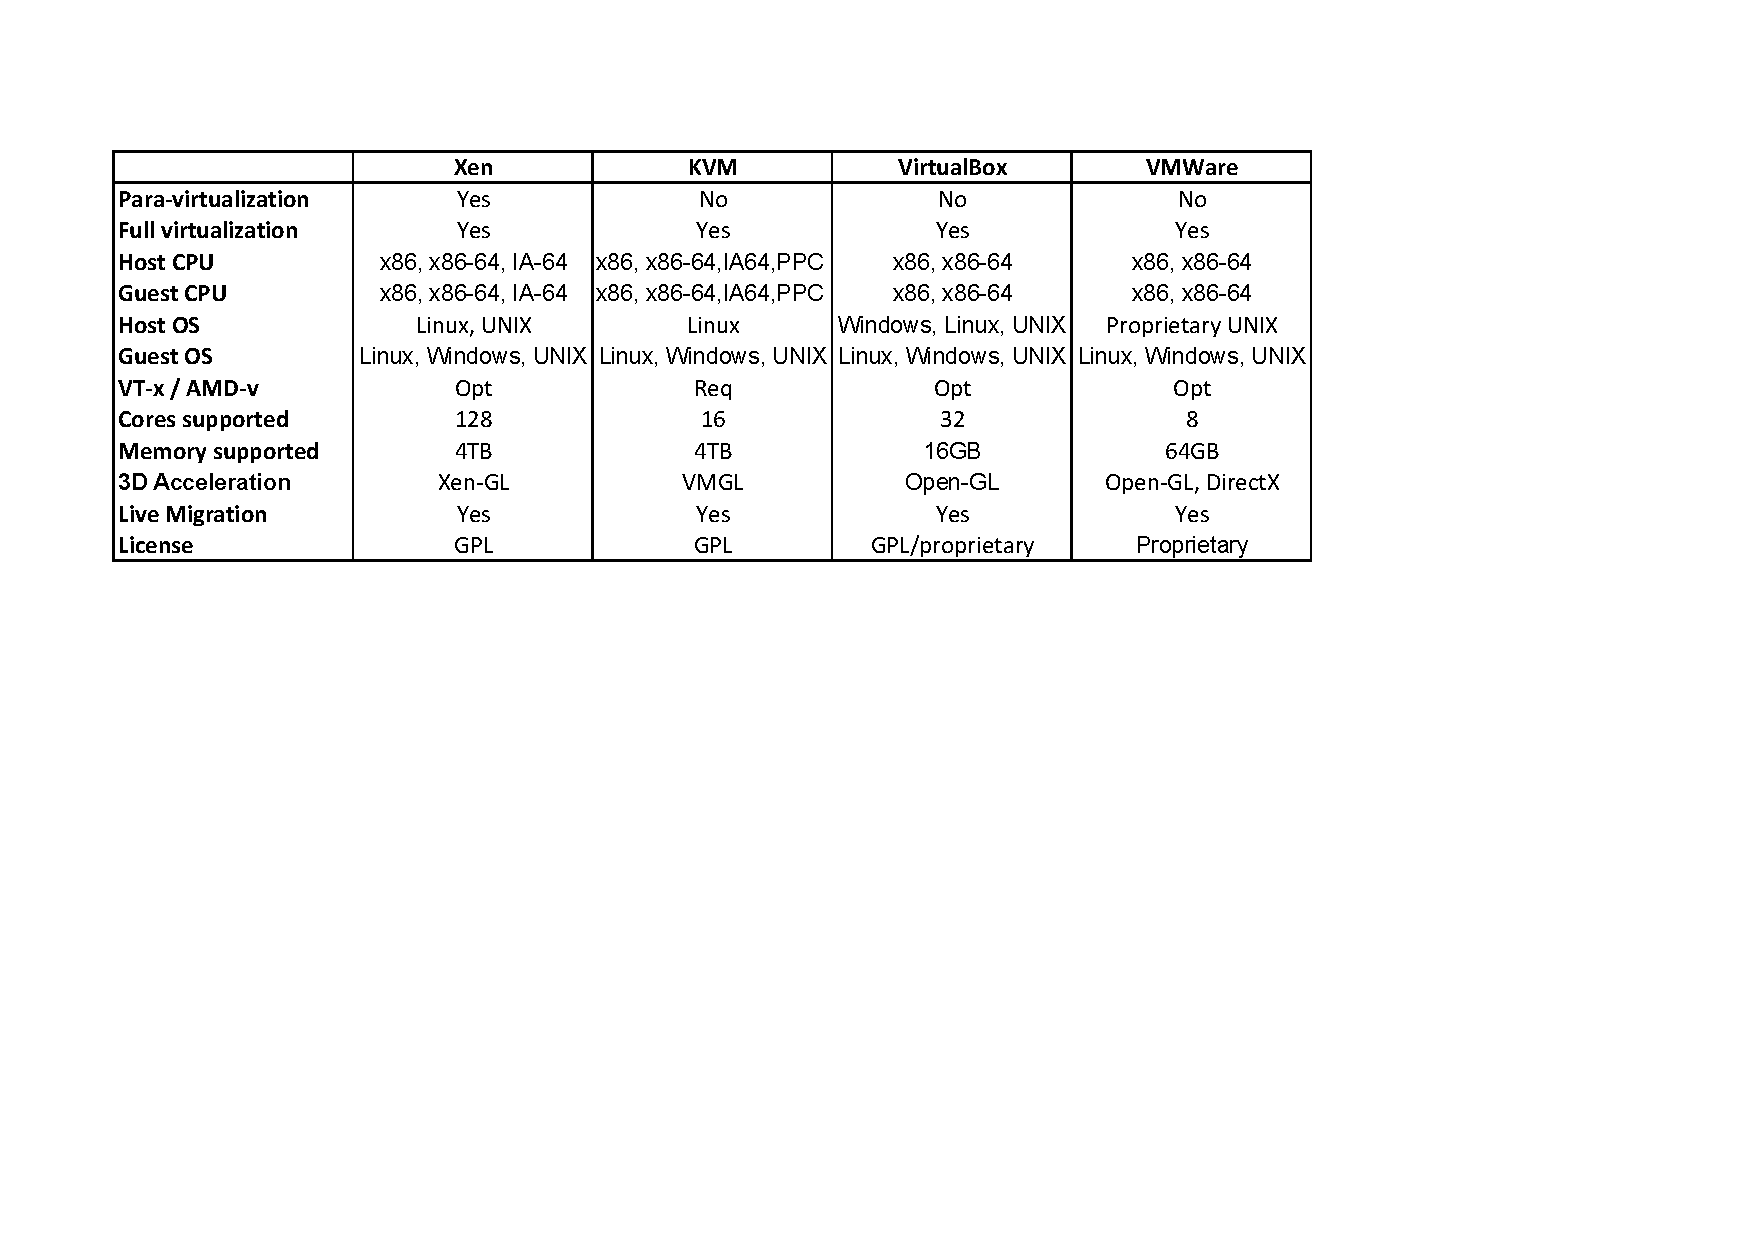
\epsfig{file=images/virt-comparison.pdf,  width=6in}
%\caption{A comparison chart between Xen, KVM, VirtualBox, and VMWare ESX} 
%\end{figure*} 


The first point of investigation is the virtualization method of each VM.  Each hypervisor supports full virtualization, which is now common  practice within most x86 virtualization deployments today.  Xen, originating as a para-virtualized VMM, still supports both types, however full virtualization is often preferred as it does not require the manipulation of the guest kernel in any way.  From the Host and Guest CPU lists, we see that x86 and, more specifically, x86-64/amd64 guests are all universally supported.  Xen and KVM both suport Itanium-64 architectures for full virtualization (due to both hypervisors dependency on QEMU), and KVM also claims support for some recent PowerPC architectures. However, we concern ourselves only with x86-64 features and performance, as other architectures are out of the scope of this manuscript.  Of the x86-64 platforms, KVM is the only hypervisor to require either Intel VT-X or AMD-V instruction sets in order to operate.  VirtualBox and VMWare have internal mechanisms to provide full virtualization even without the virtualization instruction sets, and Xen can default back to para-virtualized guests.  

Next, we consider the host environments for each system.  As Linux is the primary OS type of choice within HPC deployments, its key that all hypervisors support Linux as a guest OS, and also as a host OS. As VMWare ESX is meant to be a virtualization-only platform, it is built upon a specially configured Linux/UNIX proprietary OS specific to its needs.  All other hypervisors support Linux as a host OS, with VirtualBox also supporting Windows, as it was traditionally targeted for desktop-based virtualization.  However, as each hypervisor uses VT-X or AMD-V instructions, each can support any modern OS targeted for x86 platforms, including all variants of Linux, Windows, and UNIX. 

While most hypervisors have desirable host and guest OS support, hardware support within a guest environment varies drastically.  Within the HPC environment, virtual CPU (vCPU) and maximum VM memory are critical aspects to choosing the right virtualization technology.  In this case, Xen is the first choice as it supports up to 128 vCPUs and can address 4TB of main memory in 64-bit modes, more than any other.  VirtualBox, on the other hand, supports only 32 vCPUs and 16GB of addressable RAM per guest OS, which may lead to problems when looking to deploy it on large multicore systems.  KVM also faces an issue with the number of vCPU supported limited to 16, recent reports indicate it is only a soft limit \cite{Harper2009}, so deploying KVM in an SMP environment may not be a significant hurdle. Furthermore, all hypervisors provide some 3D acceleration support (at least for OpenGL) and support live migration across homogeneous nodes, each with varying levels of success.  

Another vital juxtaposition of these virtualization technologies is the license agreements for its applicability within HPC deployments.  Xen, KVM, and VirtualBox are provided for free under the GNU Public License (GPL) version 2, so they are open to use and modification by anyone within the community, a key feature for many potential users.  While VirtualBox is  under GPL, it has recently also offered with additional features under a more proprietary license dictated by Oracle since its acquirement from Sun last year.  VMWare, on the other hand, is completely proprietary with an extremely limited licensing scheme that even prevents the authors from willfully publishing any performance benchmark data without specific and prior approval.  As such, we have neglected VMWare form the remainder of this manuscript. Whether going with a proprietary or open source hypervisor, support can be acquired (usually for an additional cost) with ease from each option.   

\subsection{Usability}

While side by side feature comparison may provide crucial information about a potential user's choice of hypervisor, that may also be interested in its ease of installation and use.  We will take a look at each hypervisor from two user perspectives, a systems administrator and normal VM user.  

One of the first things on any system administrator's mind on choosing a hypervisor is the installation.  For all of these hypervisors, installation is relatively painless.  For the FutureGrid support group, KVM and VirualBox are the easiest of the all tested hypervisors to install, as there are a number of supported packages available and installation only requires the addition of one or more kernel modules and the support software.  Xen, while still supported in binary form by many Linux distributions, is actually much more complicated.  This is because Xen requires a full modification to the kernel itself, not just a module.  Loading a new kernel into the boot process which may complicate patching and updating later in the system's maintenance cycle.  VMWare ESX, on the other hand, is entirely separate from most other installations.  As previously noted, ESX is actually a hypervisor and custom UNIX host OS combined, so installation of ESX is likewise to installing any other OS from scratch.  This may be either desirable or adverse, depending on the system administrator's usage of the systems and VMWare's ability to provide a secure and patched environment.

While system administrators may be concerned with installation and maintenance, VM users and Cloud developers are more concerned with daily usage. The first thing to note about all of such virtualiation technologies is they are supported (to some extent) by the libvirt API \cite{Bolte2010}.  Libvirt is commonly used by many of today's IaaS Cloud offerings, including Nimbus, Eucalyptus, OpenNebula and OpenStack.  As such, the choice of hypervisor for Cloud developer's is less of an issue, so long as the hypervisor supports the features they desire.  For individual command line usage of each tool, it varies quite a bit more.  Xen does provide their own set of tools for controlling and monitoring guests, and seem to work relatively well but do incur a slight learning curve.  KVM also provides its own CLI interface, and while it is often considered less cumbersome it provides less advanced features directly to users, such as power management or quick memory adjustment (however this is subject to personal opinion).  One advantage of KVM is each guest actually runs as a separate process within the host OS, making it easy for a user to manage and control the VM inside the host if KVM misbehaves.  VirtualBox, on the other hand, provides the best command line and graphical user interface.  The CLI, is especially well featured when compared to Xen and KVM as it provides clear, decisive and well documented commands, something most HPC users and system administrators alike will appreciate.  VMWare provides a significantly enhanced GUI as well as a Web-based ActiveX client interface that allows users to easily operate the VMWare host remotely.  In summary, there is a wide variance of interfaces provided by each hypervisor, however we recommend Cloud developers to utilize the libvirt API whenever possible.  


%%%%%%%%%%%%%%%%%%%%%%%%%%%%%%%%%%%%%%%%%%%%%%%%%%%%%%%%%%%%%%%%%%%%%%
\section{Experimental Design}
%%%%%%%%%%%%%%%%%%%%%%%%%%%%%%%%%%%%%%%%%%%%%%%%%%%%%%%%%%%%%%%%%%%%%%

In order to provide an unaltered and unbiased review of these virtualization technologies for Clouds, we need to outline a neutral testing environment.  To make this possible, we have chosen to use FutureGrid as our virtualization and cloud test-bed.  


\subsection{The FutureGrid Project}

FutureGrid (FG) \cite{www-fg} provides computing capabilities that enable researchers to tackle complex research challenges related to the use and security of Grids and Clouds. These include topics ranging from authentication, authorization, scheduling, virtualization, middleware design, interface design and cybersecurity, to the optimization of Grid-enabled and cloud-enabled computational schemes for researchers in astronomy, chemistry, biology, engineering, atmospheric science and epidemiology. 

The test-bed includes a geographically distributed set of heterogeneous computing systems, a data management system that will hold both metadata and a growing library of software images necessary for Cloud computing, and a dedicated network allowing isolated, secure experiments, as seen in Figure \ref{F:3}. The test-bed supports virtual machine-based environments, as well as operating systems on native hardware for experiments aimed at minimizing overhead and maximizing performance. The project partners are integrating existing open-source software packages to create an easy-to-use software environment that supports the instantiation, execution and recording of grid and cloud computing experiments.


 \FIGURE{htb}
  {images/FG-map.pdf}
  {1.0}
  {FutureGrid Participants and Resources}
  {F:3}


One of the goals of the project is to understand the behavior and utility of Cloud computing approaches.  However, it is not clear at this time which of these toolkits will become the users' choice toolkit. FG provides the ability to compare these frameworks with each other while considering real scientific applications \cite{las2010gce}. Hence, researchers are be able to measure the overhead of cloud technology by requesting linked experiments on both virtual and bare-metal systems, providing valuable information that help decide which infrastructure suits their needs and also helps users that want to transition from one environment to the other.  These interests and research objectives make the FutureGrid project the perfect match for this work.  Furthermore, we expect that the results gleaned from this manuscript will have a direct impact on the FutureGrid deployment itself.  

\subsection{Experimental Environment}

Currently, one of FutureGrid's latest resources is the {\it India} system, a 256 CPU IBM iDataPlex machine consisting of 1024 cores, 2048 GB of ram, and 335 TB of storage within the Indiana University Data Center.  In specific, each compute node of India has two Intel Xeon 5570 quad core CPUs running at 2.93Ghz, 24GBs of Ram, and a QDR InfiniBand connection.  A total of four nodes were allocated directly from India for these experiments.  All were loaded with a fresh installation of Red Hat Enterprise Linux server 5.5 x86\_64 with the 2.6.18-194.8.1.el5 kernel patched. Three of the four nodes were installed with different hypervisors; Xen version 3.1, KVM (build 83), and VirtualBox 3.2.10, and the forth node was left as-is to act as a control for bare-metal native performance.  

Each guest virtual machine was also built using Red Hat EL server 5.5 running an unmodified kernel using full virtualization techniques.  All tests were conducted giving the guest VM 8 cores and 16GB of ram to properly span a compute node.  Each benchmark was run a total of 20 times, with the results averaged to produce consistent results, unless indicated otherwise.


\subsection{Benchmarking Setup}

As this manuscript aims to objectively evaluate each virtualization technology from a side-by-side comparison as well as from a performance standpoint, the selection of benchmarking applications is critical.  

The performance comparison of each virtual machine is based on two well known industry standard performance benchmark suites; HPCC and  SPEC. These two benchmark environments are recognized for their standardized reproducible results in the HPC communit, and the National Science Foundation (NSF), Department of Energy (DOE), and DARPA are all sponsors of the HPCC benchmarks. The following benchmarks provide a means to stress and compare processor, memory, inter-process communication, network, and overall performance and throughput of a system.  These benchmarks were selected due to their importance to the HPC community sinse they are often directly correlated with overall application performance \cite{Dujmovic1998}. 
 


\subsubsection{HPCC Benchmarks}
The HPCC Benchmarks \cite{luszczek2006hpc, Dongarra2010} are an industry standard for performing benchmarks for HPC systems. The benchmarks are aimed at testing the system on multiple levels to test their performance. It consists of 7 different tests:

\begin{itemize}
\item {\em HPL} - The Linpack TPP benchmark measures the floating point rate of execution for solving a linear system of equations.  This benchmark is perhaps the most important benchmark within HPC today, as it is the basis of evaluation for the Top 500 list \cite{www-top500}.
 \item {DGEMM} - Measures the floating point rate of execution of double precision real matrix-matrix multiplication.
\item {\em STREAM} - A simple synthetic benchmark program that measures sustainable memory bandwidth (in GB/s) and the corresponding computation rate for simple vector kernel.
\item {\em PTRANS} - Parallel matrix transpose exercises the communications where pairs of processors communicate with each other simultaneously. It is a useful test of the total communications capacity of the network.
\item {\em RandomAccess} - Measures the rate of integer random updates of memory (GUPS).
\item {\em FFT} - Measures the floating point rate of execution of double precision complex one-dimensional Discrete Fourier Transform (DFT).
\item {\em Communication bandwidth and latency} - A set of tests to measure latency and bandwidth of a number of simultaneous communication patterns; based on b\_eff (effective bandwidth benchmark).
\end{itemize}


This benchmark suite uses each test to stress test the performance on multiple aspects of the system. It also provides reproducible results which can be verified by other vendors. This benchmark is used to create the Top 500 list \cite{www-top500} which is the list of the current top supercomputers in the world. The results that are obtained from these benchmarks provide an unbiased performance analysis of the hypervisors. Our results provide insight on inter-node PingPong bandwidth, PingPong latency, and FFT calculation performance. 

\subsubsection{SPEC Benchmarks}

The Standard Performance Evaluation Corporation (SPEC) \cite{dixit1991, www-spec} is the other major standard for evaluation of benchmarking systems. SPEC has several different testing components that can be utilized to benchmark a system. For our benchmarking comparison we will use the SPEC OMP2001 because it appears to represent a vast array of new and emerging parallel applications wile simultaniously providing a comparison to other SPEC benchmarks.  SPEC OMP continues the SPEC tradition of giving HPC users the most objective and representative benchmark suite for measuring the performance of SMP (shared memory multi-processor) systems.

\begin{itemize}

\item The benchmarks are adapted from SPEC CPU2000 and contributions to its search program.
\item The focus is to deliver systems performance to real scientific and engineering applications.
\item The size and runtime reflect the needs of engineers and researchers to model large complex tasks.
\item Two levels of workload characterize the performance of medium and large sized systems.
\item Tools based on the SPEC CPU2000 toolset make these the easiest ever HPC tests to run.
\item These benchmarks place heavy demands on systems and memory.

\end{itemize}



%%%%%%%%%%%%%%%%%%%%%%%%%%%%%%%%%%%%%%%%%%%%%%%%%%%%%%%%%%%%%%%%%%%%%%
\section{Performance Comparison}
%%%%%%%%%%%%%%%%%%%%%%%%%%%%%%%%%%%%%%%%%%%%%%%%%%%%%%%%%%%%%%%%%%%%%%

The goal of this manuscript is to effectively compare and contrast the various virtualization technologies, specifically for supporting HPC-based Clouds.  The first set of results represent the performance of HPCC benchmarks.  Each benchmark was run a total of 20 times, and the mean values taken with error bars represented using the standard deviation over the 20 runs.  The benchmarking suite was built using the Intel 11.1 compiler, uses the Intel MPI and MKL runtime libraries, all set with defaults and no optimizations whatsoever.

We open first with High Performance Linpack (HPL), the de-facto standard for comparing resources.  In Figure \ref{F:hpl}, we can see the comparison of Xen, KVM, and Virtual Box compared to native bare-metal performance.  First, we see that native is capable of around 73.5 Gflops which, with no optimizations, achieves 75\% of the theoretical peak performance.  Xen, KVM and VirtualBox perform at 49.1, 51.8 and 51.3 Gflops, respectively when averaged over 20 runs.  However Xen, unlike KVM and VirtualBox, has a high degree of variance between runs.  This is an interesting phenomenon for two reasons.  First, this may impact performance metrics for other HPC applications and cause errors and delays between even pleasingly-parallel applications and add to reducer function delays.  Second, this wide variance breaks a key component of Cloud computing providing a specific and predefined quality of service.  If performance can sway as widely as what occurred for Linpack, then this may have a negative impact on users.   


 \FIGURE{htb}
  {images/linpack.png}
  {1.0}
  {Linpack performance}
  {F:hpl}


Next, we turn to another key benchmark within the HPC community, Fast Fourier Transforms (FFT).  Unlike the synthetic Linpack benchmark, FFT is a specific, purposeful benchmark which provides results which are often regarded as more relative to a user's real-world application than HPL.  From Figure \ref{F:fft}, we can see rather distinct results from what was previously provided by HPL. Looking at Star and Single FFT, its clear performance across all hypervisors is roughly equal to bare-metal performance, a good indication that HPC applications may be well suited for use on VMs.  The results for MPI FFT also show similar results, with the exception of Xen, which has a decreased performance and high variance as seen in the HPL benchmark.  Our current hypothesis is that there is an adverse affect of using Intel's MPI runtime on Xen, however the investigation is still ongoing.

\FIGURE{htb}
  {images/FFT.png}
  {1.0}
  {Fast Fourier Transform performance}
  {F:fft}


Another useful benchmark illustrative of real-world performance between bare-metal performance and various hypervisors are the ping-pong benchmarks.  These benchmarks measure the bandwidth and latency of passing packets between multiple CPUs.  With this experiment, all ping-pong latencies are kept within a given node, rather than over the network.  This is done to provide further insight into the CPU and memory overhead withing each hypervisor.  From Figure \ref{F:ppb} the intranode bandwidth performance is uncovered, with some interesting distinctions between each hypervisor.  First, Xen performs, on average, close to native speeds, which is promising for the hypervisor.  KVM, on the other hand, shows consistent overhead proportional to native performance across minimum, average, and maximum bandwidth.  VirtualBox, on the other hand, performs well, in fact too well to the point that raises alarm.  While the minimum and average bandwidths are within native performance, the maximum bandwidth reported by VirtualBox is significantly greater than native measurements, with a large variance.  After careful examination, it appears this is due to how VirtualBox assigns its virtual CPUs.  Instead of locking a virtual CPU to a real CPU, a switch may occur which could benefit on the off-chance the two CPU's in communication between a ping-pong test could in fact be the same physical CPU.  The result would mean the ping-pong packet would remain in cache and result in a higher perceived bandwidth than normal.  While this effect may be beneficial for this benchmark, it may only be an illusion towards the real performance gleaned from the VirtualBox hypervisor. 

\FIGURE{htb}
  {images/pingpongbandwidth.png}
  {1.0}
  {Ping Pong bandwidth performance}
  {F:ppb}

The Bandwidth may in fact be important within the ping-ping benchmark, but the latency between each ping-pong is equally useful in understanding the performance impact of each virtualization technology.  From Figure \ref{F:ppl}, we see KVM and VirtualBox have near-native performance; another promising result towards the utility of hypervisors within HPC systems.  Xen, on the other hand, has extremely high latencies, especially at for maximum latencies, which in turn create a high variance within the average latency within the VM's performance.  


\FIGURE{htb}
  {images/pingponglatency.png}
  {1.0}
  {Ping Pong latency performance (lower is better)}
  {F:ppl}



While the HPCC benchmarks provide a comprehensive view for many HPC applications including Linpack and FFT using MPI, performance of intra-node SMP applications using OpenMP is also investigated.  Figure \ref{F:specomp} illustrates SPEC OpenMP performance across the VMs we concentrate on, as well as baseline native performance.  First, we see that the combined performance over all 11 applications executed 20 times yields the native testbed with the best performance at a SPEC score of 34465.  KVM performance comes close with a score of 34384, which is so similar to the native performance that most users will never notice the difference.  Xen and VirtualBox both perform notably slower with scores of 31824 and 31695, respectively, however this is only an 8\% performance drop compared to native speeds. Further results can be found on the SPEC website \cite{spec2011}. 

\FIGURE{htb}
  {images/spec-omp.png}
  {1.0}
  {Spec OpenMP performance}
  {F:specomp}

%%%%%%%%%%%%%%%%%%%%%%%%%%%%%%%%%%%%%%%%%%%%%%%%%%%%%%%%%%%%%%%%%%%%%%
\section{Discussion}
%%%%%%%%%%%%%%%%%%%%%%%%%%%%%%%%%%%%%%%%%%%%%%%%%%%%%%%%%%%%%%%%%%%%%%

The primary goal of this manuscript is to evaluate the viability of virtualization within HPC.  After our analysis, the answer seems to be a resounding "yes."  However, we also hope to select the best virtualization technology for such an HPC environment.  In order to do this, we combine the feature comparison along with the performance results, and evaluate the potential impact within the FutureGrid testbed.    

From a feature standpoint, most of today's virtualization technologies fit the bill for at least small scale deployment, including VMWare.  In short, each support Linux x86\_64 platforms, use VT-X technology for full virtualization, and support live migration.  Due to VMWare's limited and costly licensing, it is immediately out of contention for most HPC deployments.  From a CPU and memory standpoint, Xen seems to provide the best expandability, supporting up to 128 cpus and 4TB of addressable RAM.  So long as KVM's vCPU limit can be extended, it too shows promise as a feature-full virtualization technology.  One of Virtualbox's greatest limitations was the 16GB maximum memory allotment for individual guest VMs, which actually limited us from giving VMs more memory for our performance benchmarks. If this can be fixed and Oracle does not move the product into the proprietary market, VirtualBox may also stand a chance for deployment in HPC environments.  


\FIGURE{htb}
  {images/benchmark-summary.pdf}
  {1.0}
  {Benchmark rating summary (lower is better)}
  {F:summary}


From the benchmark results previously described, the use of hypervisors within HPC-based Cloud deployments is mixed batch.  Figure \ref{F:summary} summarizes the results based on a 1-3 rating, 1 being best and 3 being worst.   While Linpack performance seems to take a significant performance impact across all hypervisors, the more practical FFT benchmarks seem to show little impact, a notably good sign for virtualization as a whole.  The ping-pong bandwidth and latency benchmarks also seem to support this theory, with the exception of Xen, who's performance continually  has wide fluctuations throughout the majority of the benchmarks.  OpenMP performance through the SPEC OMP benchmarking suite also shows promising results for the use of hypervisors in general, with KVM taking a clear lead by almost matching native speeds. 

While Xen is typically regarded as the most widely used hypervisor, especially within academic clouds and grids, it's performance has shown lack considerably when compared to either KVM or VirtualBox.  In particular, Xen's wide and unexplained fluctuations in performance throughout the series of benchmarks suggests that Xen may not be the best choice for building a lasting quality of service infrastructure upon. From Figure \ref{F:summary}, KVM rates the best across all performance benchmarks, making it the optimal choice for {\em general} deployment in an HPC environment.  Furthermore, this work's illustration of the variance in performance among each benchmark and the applicability of each benchmark towards new applications may make possible the ability to preemptively classify applications for accurate prediction towards the ideal virtualized Cloud environment. We hope to further investigate this concept through the use of the FutureGrid experiment management framework at a later date.


In conclusion, it is the authors' projection that KVM is the best overall choice for use within HPC Cloud environments. KVM's feature-rich experience and near-native performance makes it a natural fit for deployment in an environment where usability and performance are paramount.  Within the FutureGrid project specifically, we hope to deploy the KVM hypervisor across our Cloud platforms in the near future, as it offers clear benefits over the current Xen deployment.  Furthermore, we expect these findings to be of great importance to other public and private Cloud deployments, as system utilization, Quality of Service, operating cost, and computational efficiency could all be improved through the careful evaluation of underlying virtualization technologies. 





